\documentclass[kulak]{kulakposter}
\usepackage[dutch]{babel}
\usepackage{graphicx}
\usepackage{amsmath}
\usepackage{hyperref}

\faculty{Teamopdracht 2023 -- 2024}
\title{Classificatie met lineaire Support Vector Machines}
\author{Team \(\exists\)uler}
\institute{Vincent Van Schependom, Daan Vanhaverbeke, Jasper Benoit, Lasha Shergelashvili, Marie Taillieu, Zeineb Kharbach, Florian Degraeve, Younes Mebarki}
\photo{groepsfoto}

\newcommand{\norm}[1]{\left\| #1 \right\|}
\renewcommand{\boxed}[1]{\text{\fboxsep=.3em\fbox{#1}}}

\begin{document}

\maketitle

\begin{multicols}{2}
	\section*{Inleiding}
	\vspace{0.5cm}
	SVM of \textbf{Support Vector Machines} is een classificatietechniek.
	
	\begin{multicols}{2}
		Dataset met \(p\) verschillende \textit{features}:
		\begin{itemize}
			\item \((p-1)\)-dimensionele hypervlakken
			\item Deze splitsen de dataset in twee groepen
		\end{itemize}
		\columnbreak
		
		\textbf{Binaire} classificatie (\(><\) \textit{multi-class}):
		\begin{itemize}
			\item Een punt behoort tot een van twee klassen
			\item \(y \in \{-1,1\}\)
		\end{itemize}
	\end{multicols}
	
	\vspace{0.5cm}
	\centering
	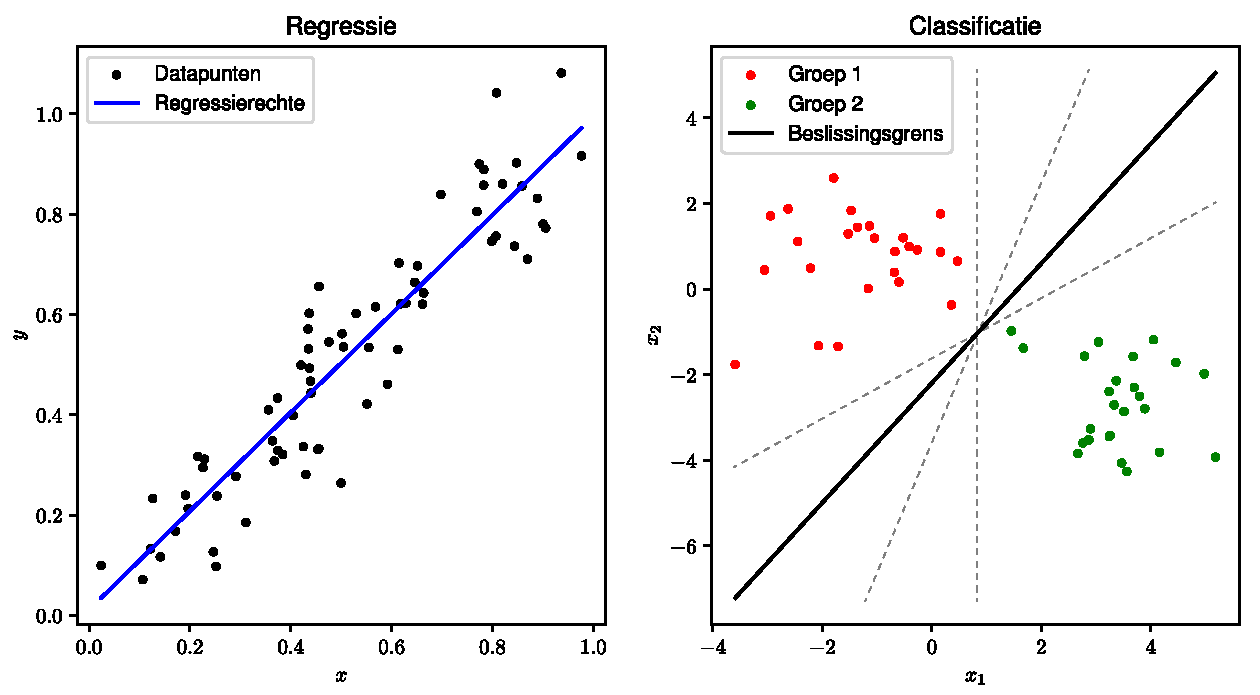
\includegraphics[width=.95\columnwidth]{regressievsclassificatie}
	
	\columnbreak
	\section{\textit{Maximum margin} hypervlakken}
	\vfill \null
		\begin{multicols}{2}
			\setlength\columnsep{0cm}
			\photohere
			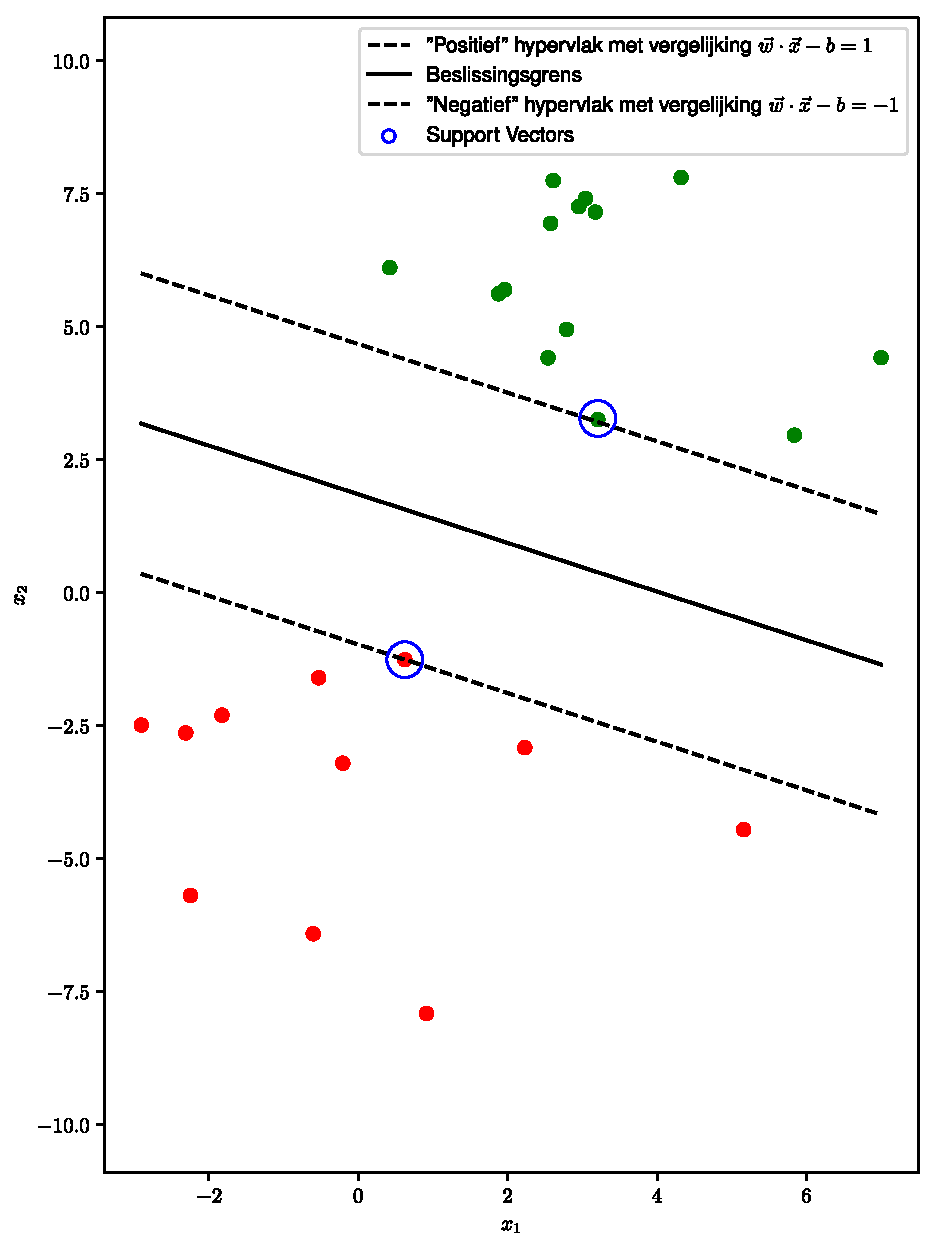
\includegraphics[width=.90\columnwidth]{svm}
			
			\columnbreak
			
			\vspace{1cm} \null
			
			We definiëren twee lineaire \textbf{hypervlakken}:
			\begin{center}
				\(\vec{w} \cdot \vec{x} - b = 1 \quad \text{en} \quad \vec{w} \cdot \vec{x} - b = -1\)
			\end{center}
			
			\vspace{0.3cm}

			Aangezien er \textbf{twee features} zijn:
			\begin{center}
				\(w_1x_1 + w_2x_2 - b = 1 \quad \text{en} \quad w_1x_1 + w_2x_2 - b = -1\)
			\end{center}
			
			\vspace{1cm}
			
			\begin{itemize}
				\item \(\vec{w}\) is de \textbf{normaalvector} op de hypervlakken
				\item \(b\) is de \textit{\textbf{intercept}} van de rechte die de\\ beslissingsrechte beschrijft
				\item De punten die op/in de marge ligggen, \\heten de \textbf{\textit{support vectors}}
				\item De \textbf{beslissingsgrens} ligt in het midden van beide hypervlakken
				\item Maximalisatie van de \textbf{marge}\\
				
			\end{itemize}
			
			\vspace{0.5cm} \null
			
		\end{multicols}
		
		\vspace{0.5cm}
		
		\centering
		\(\frac{2}{\norm{\vec{w}}}\) maximaliseren \(\Rightarrow\) \(\norm{\vec{w}}\) minimaliseren
		
		\vfill \null
	
\end{multicols}
	
\begin{multicols}{2}
	
	\section{\textit{Hinge loss} \(l\)}
	
	De \textbf{\textit{hinge loss}} is een soort foutterm die als volgt gedefinieerd wordt:
	\[l=\max{(0,1-y_i(\vec{w}\cdot\vec{x}_i-b))}\]
	
	\vspace{0.5cm}
	
		\textbf{Goed geclassificeerde punten:}
		\begin{itemize}
			\item Aan de juiste kant van het positief/negatief hypervlak
			\item 	\(\left. \begin{array}{ll}
				\vec{w}\cdot \vec{x}_i-b\geq 1 & \text{als } y_i=1 \\
				\vec{w}\cdot \vec{x}_i-b\leq -1 & \text{als } y_i=-1
			\end{array} \right\} \Rightarrow y_i(\vec{w}\cdot \vec{x}_i-b)\geq 1 \Rightarrow \boxed{$l=0$} \)
		\end{itemize}
		\vspace{0.5cm}
		\textbf{Slecht geclassificeerde punten:}\\
		Twee opties:
		\begin{itemize}
			\item In de marge \(\Rightarrow\) \boxed{$0<l\leq 1$}
			\item Aan de foute kant van de beslissingsgrens \(\Rightarrow\) \boxed{$l > 1$}
		\end{itemize}
	
\section{Kostfunctie \(J\)}
\begin{multicols}{2}
	Optimaal model:
	\begin{itemize}
		\item Maximale marge \(\rightarrow\) minimale \(\norm{\vec{w}}\)
		\item Maximale accuraatheid \(\rightarrow\) minimale \(l\)
	\end{itemize}
	\columnbreak
	Kostfunctie \(J\) minimaliseren:
	\[\min_{w,b}J=\min_{w,b}\left(\frac{1}{n} \sum_{i=1}^n{\max{l_i}} + \lambda\cdot{||\vec{w}||}^2\right)\]
\end{multicols}

\columnbreak

\section{Regularisatieparameter \(\lambda\)}

De metaparameter wordt bij SVM de \textbf{regularisatieparameter} genoemd, aangeduid met \(\lambda\).

Deze \(\lambda\) heeft invloed op de minimalisatie van \(J\):

\begin{itemize}
\item Kleine \(\lambda\) \(\rightarrow\) zo veel mogelijk \textit{hinge losses} op 0 zetten \(\rightarrow\) \boxed{kleine marge} 
\item Grote \(\lambda\) \(\rightarrow\) meer nadruk op het minimaliseren van de grootte van \(\norm{\vec{w}}\) \(\rightarrow\) \boxed{grote marge}
\end{itemize}

\photohere
\centering
\includegraphics[width=.98\columnwidth]{regularisatieparameter}

\end{multicols}
\section{Voordelen van tegenover andere classificatietechnieken}
	
	\begin{multicols}{3}
		
		\vfill \null
		
		\begin{center}
		\textit{Hinge loss} is een \textbf{goede \textit{loss}-functie}\\
		\includegraphics[width=.99\columnwidth]{lossfuncties}
		\end{center}
		
		\columnbreak
		
		\vfill \null
		
		\textit{Support vectors}:\\ \(\rightarrow\) SVM is niet gevoelig aan \textit{\textbf{outliers}}
		
		Maximale marge:\\ \(\rightarrow\) SVM zal niet snel \textbf{\textit{overfitten}}\\
		
		\begin{center}
			\includegraphics[width=.99\columnwidth]{outlier}
		\end{center}
		
		\vfill \null
		
		\columnbreak
		
		\vfill \null
		
		\centering
		SVM werkt goed in \textbf{hogere dimensies} (3D+):\\
		\includegraphics[width=.9\columnwidth]{3d}
		
	\end{multicols}


\section*{Besluit}

Dankzij de \textit{maximum margin} hypervlakken bieden Support Vector Machines heel wat voordelen tegenover andere classificatietechnieken. De maximalisatie van de marge beschermt het model tegen \textit{overfitting}. De \textit{hinge loss}, die vervat zit in de kostfunctie, is uniek voor SVM en zorgt ervoor dat het model minder gevoelig is voor \textit{outliers}. Daarom worden Support Vector Machines ook verkozen indien de dataset eerder klein is. Ondanks het feit dat we hogere dimensies niet visueel kunnen voorstellen, zal SVM hier goed presteren.

\nocite{mediumarticle}
\nocite{Ramo_2017}

\bibliography{referenties}
\bibliographystyle{unsrt}

\end{document}
